\section{Algorithms}
  \subsection{A*}
A* use a function to determine the order in which the search visits nodes in the tree. This function is $f(x) = g(x) + h(x)$ where $g(x)$ is the path cost from the starting node to the current node and $h(x)$ is an admissible heuristic function. A* choose the next unvisited node where the function $f(x)$ is the minimum.
  
An admissible heuristic function means if $h(x) \leq r(x)$ where $r(x)$ is the cost of the path between the node $x$ and the goal node. In the vacuum world, to search a path between a cell to another, an admissible heuristic could be the Manhattan distance.

Let's take the graph below. We want to go from node A to node D. An admissible function h could be :
$h(B) = 12$,
$h(C) = 7$,
$h(D) = 0$,
$h(E) = 10$,
$h(F) = 2$,
$h(G) = 5$

\begin{figure}[!h]
  \centering
  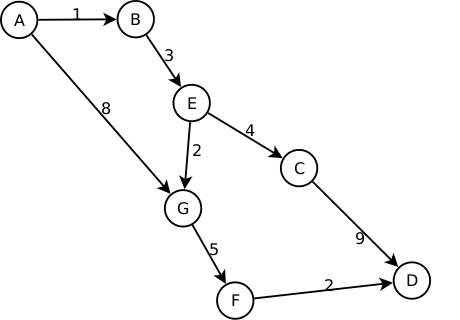
\includegraphics[height=6cm]{img/AStar_exemple.png}
  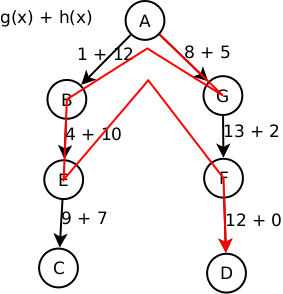
\includegraphics[height=6cm]{img/AStar_tree.png}
  \caption{Graph and it's A* exploration tree}
  \label{BFS_Levels}
\end{figure} 

Here we can see that the solution is not optimal. It's because the heuristic is not consistent ( $h(B) > cost(B,E) + h(C)$).

Using a consistent heuristic with A* assure to find the optimal path.

  \subsection{Breadth First Search}
BFS will explore the graph using a queue (FIFO), that imply that node who are the nearest (not in real cost, but in number of nodes to go across) will be explore first. The graph will be explored level by level.
We can see this exploration on the image below :

\begin{figure}[!h]
  \centering
  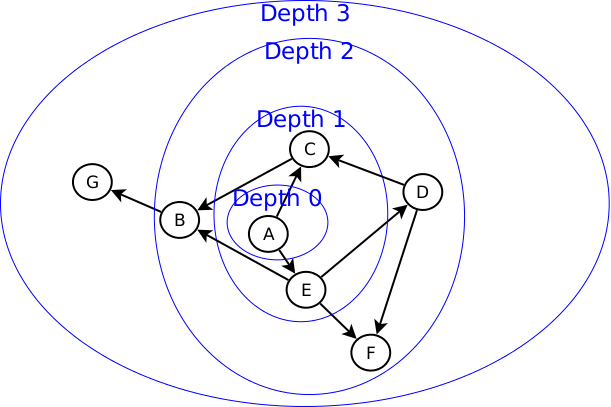
\includegraphics[height=8cm]{img/BFS_Levels.png}
  \caption{BFS exploration levels}
  \label{BFS_Levels}
\end{figure} 

Here are the way how BFS explore the tree.

\begin{figure}[h!]
  \centering
  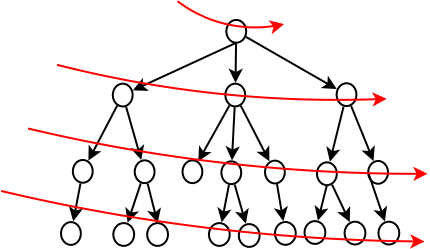
\includegraphics[height=6cm]{img/BFS_explo.png}
  \caption{BFS exploration}
\end{figure} 

BFS is a blind-search algorithm, so he don't take of the path cost during his exploration.

  \subsection{Iterative Depth First Search}

The Iterative deepening search algorithm is an extension to the Depth Limited Search algorithm.

This algorithm start with a depth threshold of 1 and execute a Depth Limited Search algorithm. If no goal node has been found, then the algorithm increase the depth threshold and re-execute a Depth Limited Search with this new threshold. The algorithm iterate until he found a goal node. Here are the way how Iterative Deepening explore the tree.

\begin{figure}[h!]
  \centering
  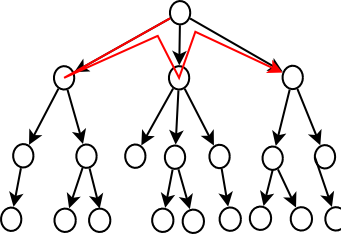
\includegraphics[height=4cm]{img/Ite_explo1.png}
  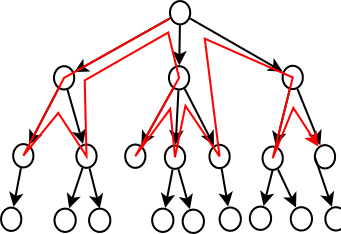
\includegraphics[height=4cm]{img/Ite_explo2.png}
  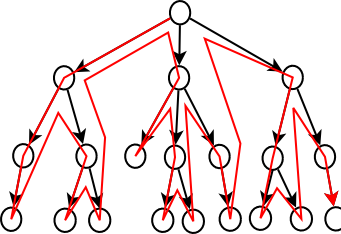
\includegraphics[height=4cm]{img/Ite_explo3.png}
  \caption{Iterative deepening (Depth threshold respectively 1, 2 and 3)}
\end{figure} 

Iterative Deepening Search is also a blind-search algorithm, so he don't take of the path cost during his exploration.

\clearpage
